\begin{figure}[H]
    \centering
        \begin{tikzpicture}[
            font={\footnotesize},
            trap/.style={trapezium, rotate=-90,trapezium angle=75},
        ]
            %% Nodes
            \node(input) at (-6, 0) {
\includegraphics[width=.1\textwidth]{fig/rel/images/cat_v2.jpg}};
            \node[above] at (input.north) {Input image $\vumod$};
            \node[draw, trap](cnn) at (-3, 0) {\rotatebox{90}{\parbox{1.0cm}{\centering{\Th{CNN}}}}};
            \node(fmaps) at (-0.5,0) {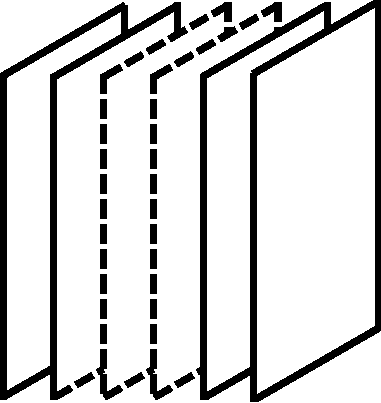
\includegraphics[width=.1\textwidth]{fig/rel/images/fmaps_side.pdf}};
            \node(fmk) at (-0.5, 1.3) {$A^k_\ell$};
            \node(classtag) at (3, 1.3) {\Th{Classifier}};
            \node(GAP) at (1.25,0.25) {$\gap$};
            \node(gapclass) at (3, 0) {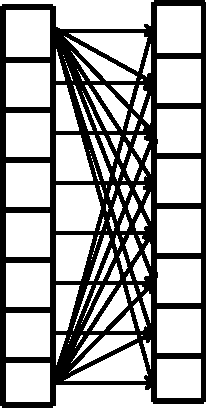
\includegraphics[width=.075\textwidth]{fig/rel/images/gapclass.pdf}};
            \node(logit) at (5, 0) {$\vy_c$};
            \node(wck) at (-0.5, -3) {
\includegraphics[width=0.02\textwidth, angle=90]{fig/rel/images/classifier.pdf}};
            \node(comb) at (-0.5, -3.5) {Weighting coefficient $w_k^c$};
            \node[draw, circle] (odot) at (-0.5, -1.8) {$\times$};
            \node(salient) at (-3, -1.8) {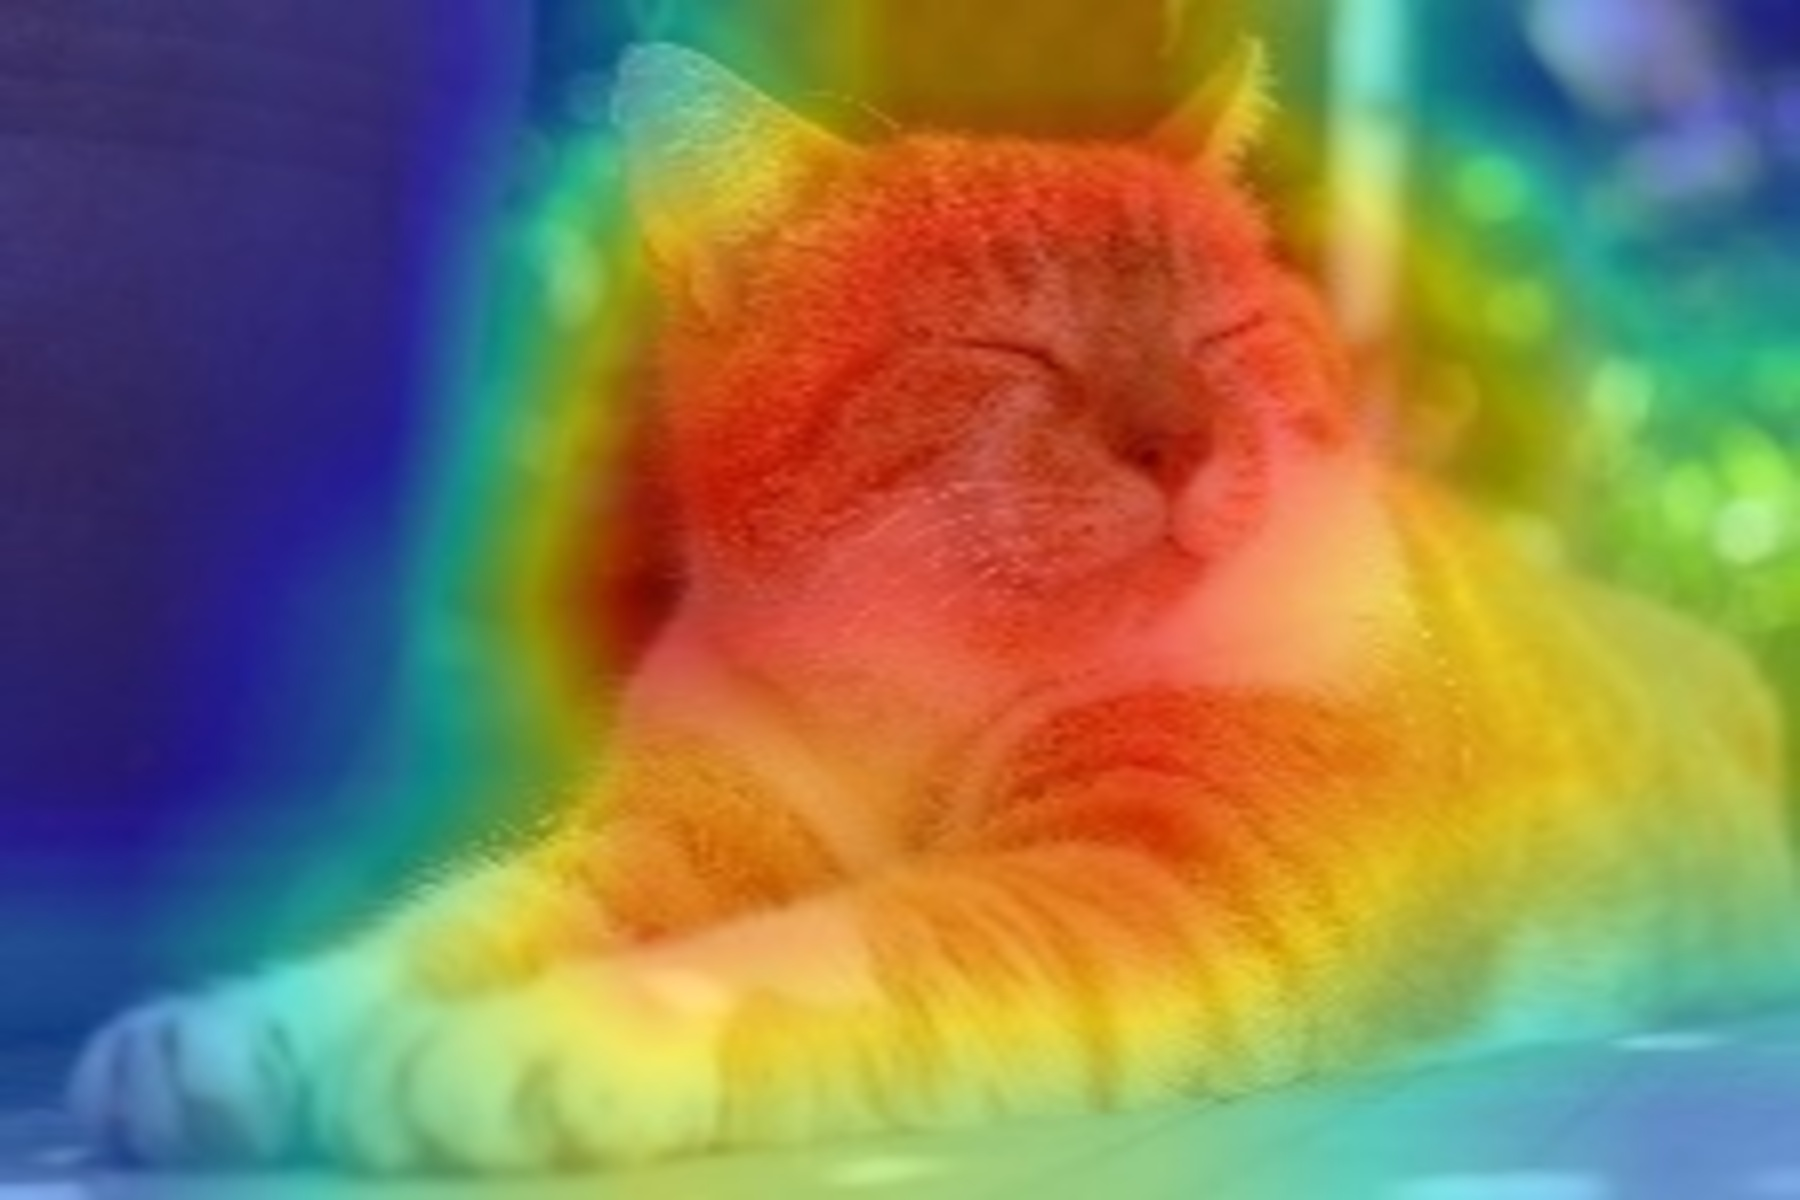
\includegraphics[width=.1\textwidth]{fig/rel/images/cat_cam.jpg}};
            \node[below] at (salient.south) {Saliency map $\mathbf{S_\ell}$};
            
            %% Edges

            \draw[->] (input.east) -- node {} (cnn);
            \draw[->] (cnn.north) -- node[above] {$\ell$} (fmaps.west);
            \draw[->] (fmaps.east) -- node {} (gapclass.west);
            \draw[->] (gapclass.east) -- node[above] {} (logit.west);
            \draw[->] (fmaps.south) -- node {} (odot.north);
            \draw[->] (wck.north) -- node {} (odot.south);
            \draw[->] (odot.west) -- node {} (salient);           

    \end{tikzpicture}
    \label{fig:cam_schema}
    \caption{\gls{cam} based methodologies overview.}
\end{figure}